\chapter{State of the Art}
\label{ch:state_of_the_art}

\paragraph*{Standard terminology}
\begin{figure}
    \centering
    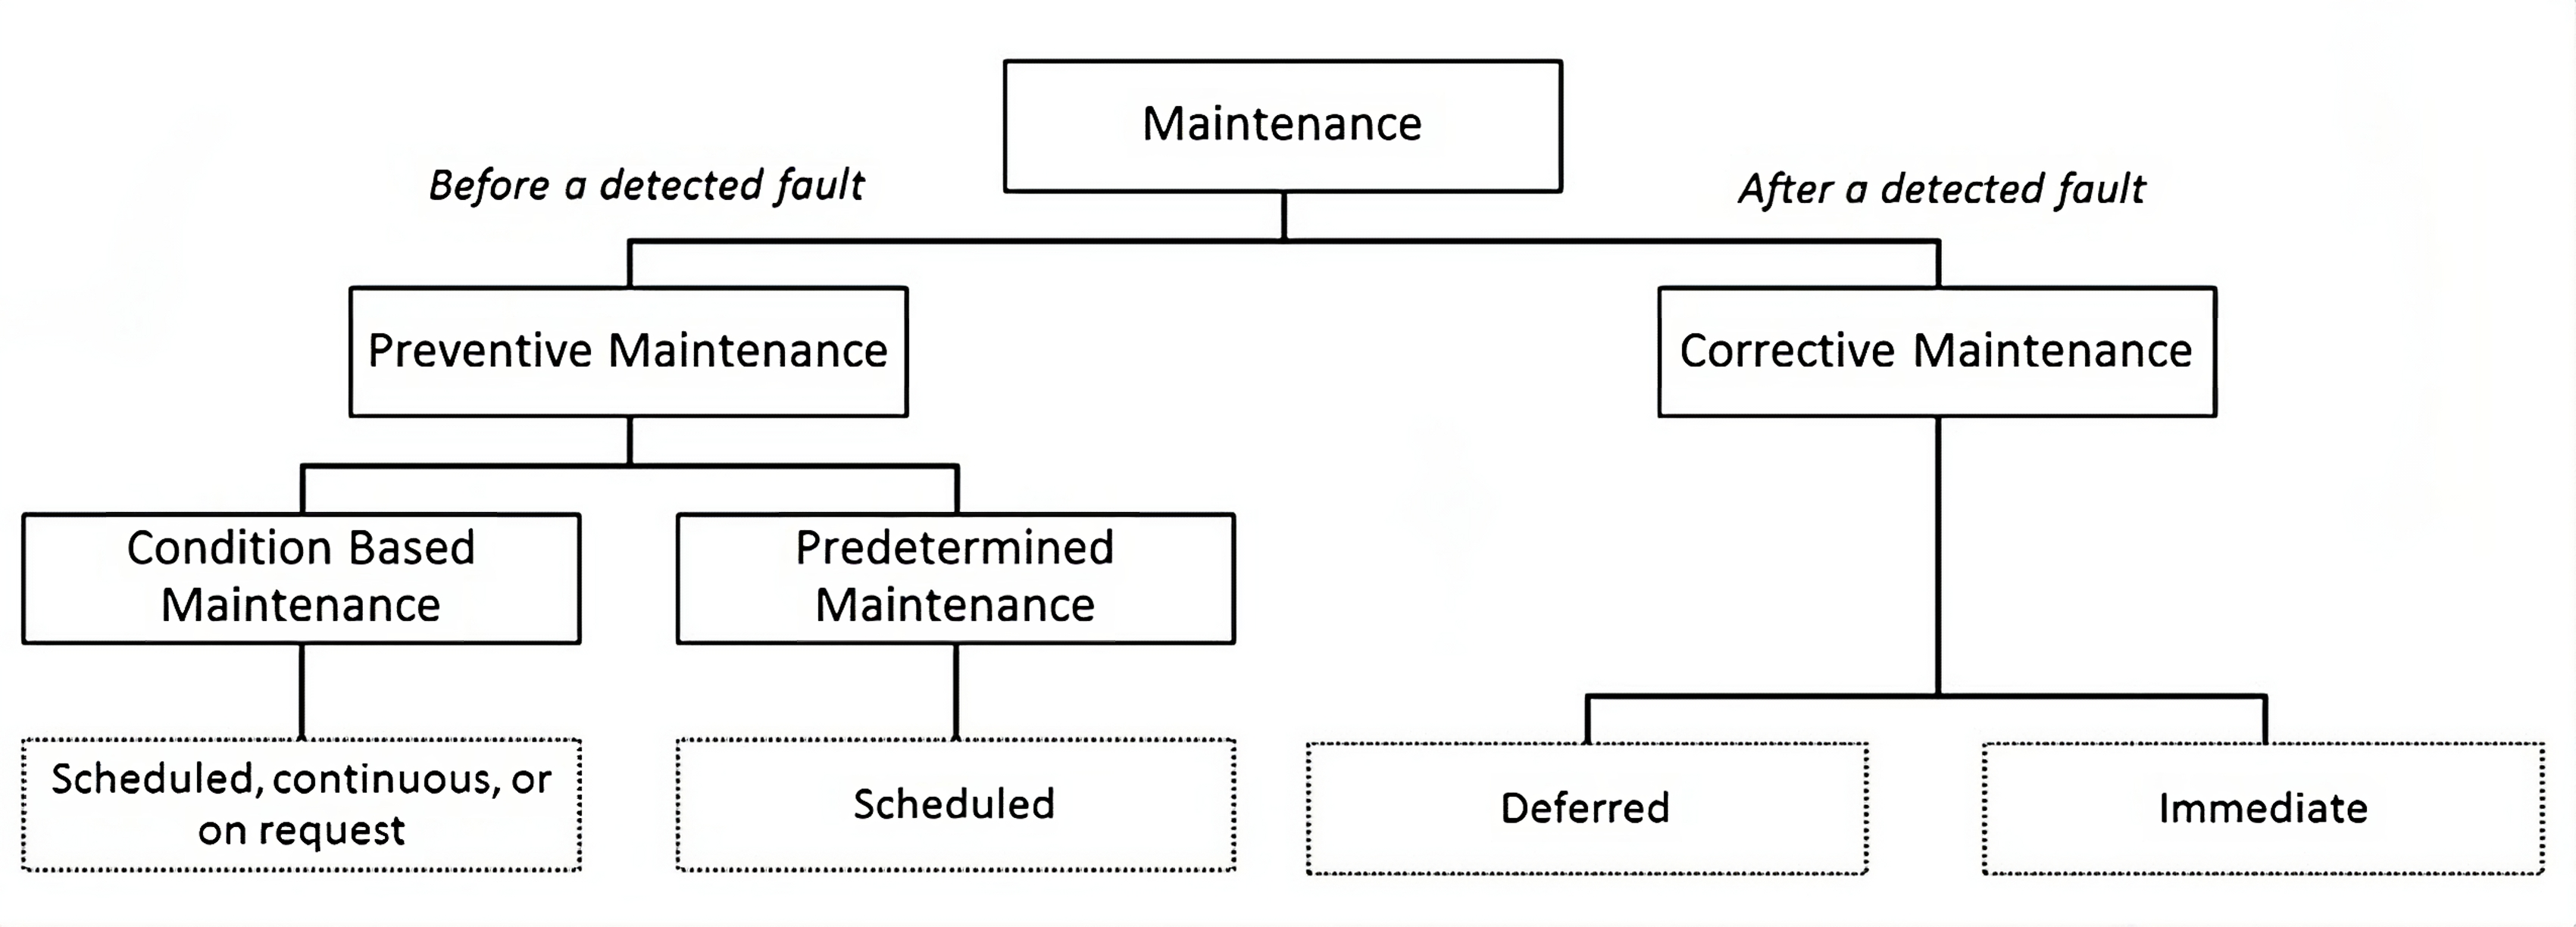
\includegraphics[width=\textwidth]{images/StateArt/EN13306.png}
    \caption{Standard terminology for industrial maintenance \cite{rastegari2017condition}}
    \label{fig:standard_terminology}
\end{figure}

A standard terminology used for industrial maintenance is provided by european committee for standardization with the standard \texttt{EN13306:2018} \cite{EN13306:2018}. The terminology is summarized in \autoref{fig:standard_terminology}. The most advanced maintenance technique family is \textbf{\gls{glo:conditionbasedmaintenance}}. This category include the most modern \textbf{\gls{glo:predictivemaintenance}}. Note that the definition does not imply that the \quoted{monitoring} of the system must be continuous, it may also be scheduled or not even scheduled.

The standard also defines what \textbf{\gls{glo:onlinemaintenance}} and \textbf{\gls{glo:onistemaintenance}}. All this definitions are reported in the {glossary}






\paragraph*{\gls{rm} vs \gls{pm}}
\begin{figure}
    \centering
    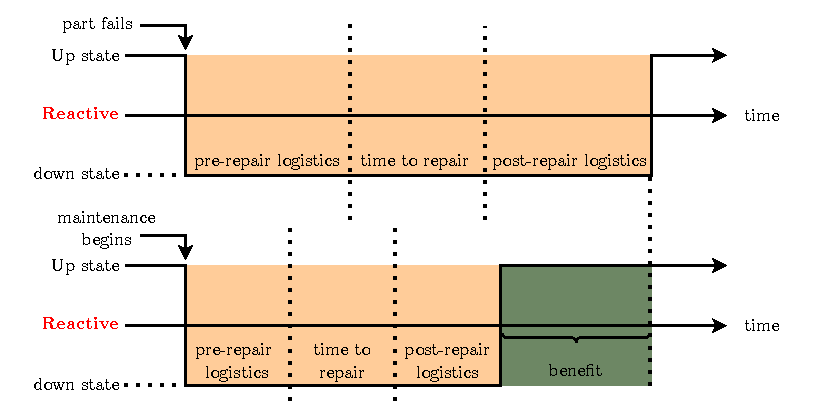
\includegraphics[scale=0.9]{images/StateArt/lost_opportunities.pdf}
    \caption{Downtime comparison (\gls{rm} and \gls{pm})}
    \label{fig:lost_opportunities}
\end{figure}

As anticipated in the introduction, the two main approaches are \textbf{reactive maintenance} (\gls{glo:correctivemaintenance} for the standard), which restores system functionality, and \textbf{proactive maintenance} (\gls{glo:correctivemaintenance} for the standard), which preserves system functionality \cite{Rely_maint_book}.

The former approach leads to very high downtime \gls{wrt} the latter \cite{NIST}. For all the time a system is down, the company forfeits the opportunity to make a profit. This is called \emph{lost opportunity cost}. In reality, the total costs of downtime are even higher, because there are other costs associated with labor overhead and materials \cite{Lost_Opport_Cost}. The second approach optimizes both the pre-repair and post-repair logistics and, acting before the failure, can reduce also the total downtime. This benefit is shown in \autoref{fig:lost_opportunities}. Other than the downtime, a more complete comparison between the advantages and disadvantages of the two approaches is shown in \autoref{tab:PM_vs_RM}.

% \usepackage{array}
% \usepackage{booktabs}


\begin{table}
    \centering
    \caption{Advantages and disadvantages of \gls{rm} and \gls{pm} maintenance \cite{Lost_Opport_Cost}}
    \resizebox{0.999999\textwidth}{!}{%
    \begin{tabular}{>{\hspace{0pt}}m{0.2\linewidth}>{\hspace{0pt}}m{0.344\linewidth}>{\hspace{0pt}}m{0.39\linewidth}} 
    \toprule
    \textbf{Maintenance} & \textbf{Advantages}                                                                                                                                                                                                                                                                                                                                                                                                                                                                                                                                                                                                                                                                                                                                                                                                                                                                                                                                  & \textbf{Disadvantages}                                                                                                                                                                                                               \\ 
    \hline
    Reactive             & \begin{tabular}{@{\labelitemi\hspace{\dimexpr\labelsep+0.5\tabcolsep}}l@{}}low setup cost\\easy to setup\end{tabular}                                                                                                                                                                                                                                                                                                                                                                                                                                                                                                                                                                                                                                                                                                                                                                                                                                & \begin{tabular}{@{\labelitemi\hspace{\dimexpr\labelsep+0.5\tabcolsep}}l@{}}unscheduled downtime\\increased labour costs\\unoptimized resources\\\begin{tabular}[c]{@{}l@{}}Increased manufacturing\\costs\end{tabular}\end{tabular}  \\ 
    \hline
    Proactive            & \begin{tabular}{@{}l@{}}{\labelitemi}\hspace{\dimexpr\labelsep+0.5\tabcolsep}\begin{tabular}[c]{@{}l@{}}increases system\\availability\end{tabular}\\{\labelitemi}\hspace{\dimexpr\labelsep+0.5\tabcolsep}\begin{tabular}[c]{@{}l@{}}minimizes logistical\\downtime\end{tabular}\\{\labelitemi}\hspace{\dimexpr\labelsep+0.5\tabcolsep}\begin{tabular}[c]{@{}l@{}}reduces unscheduled\\downtime\end{tabular}\\{\labelitemi}\hspace{\dimexpr\labelsep+0.5\tabcolsep}~decreases costs\\\hspace{0.5\leftmargin}{\labelitemii}\hspace{\dimexpr\labelsep+0.5\tabcolsep}optimizes parts\\\hspace{0.5\leftmargin}{\labelitemii}\hspace{\dimexpr\labelsep+0.5\tabcolsep}optimizes labour\\{\labelitemi}\hspace{\dimexpr\labelsep+0.5\tabcolsep}\begin{tabular}[c]{@{}l@{}}maintenance events\\planned\end{tabular}\\{\labelitemi}\hspace{\dimexpr\labelsep+0.5\tabcolsep}\begin{tabular}[c]{@{}l@{}}optimize logistical\\support~~\end{tabular}\end{tabular} & \begin{tabular}{@{\labelitemi\hspace{\dimexpr\labelsep+0.5\tabcolsep}}l@{}}high setup cost\\\begin{tabular}[c]{@{}l@{}}savings not seen\\immediately\end{tabular}\\not feasible forall equipment~\end{tabular}                       \\
    \bottomrule
    \end{tabular}
    }
    \end{table}

\paragraph*{Passive vs active maintenance}
\gls{pdm} techniques can be divided also into \emph{passive} and \emph{active}. The former uses existing sensors or add new sensors to the system and this data are just analyzed. The latter, instead, uses actuators to perturb the system and then analyzes the response. The former is more common, because it is less expensive and less invasive. The latter, instead, is more accurate but it's application is limited to special applications. The mosto common field of application of active \gls{pdm} is electrical systems, where the perturbation can be applied by injecting a current or a voltage \cite{State_Art_Hasemian_2011}.

In \cite{State_Art_Hasemian_2011}, the author gives also, as an example of active \gls{pdm}, the use the Loop Current Step Response \gls{lcsr} technique. In this test, an electrical signal in the form of a step change is sent to the sensor using a Wheatstone bridge, causing heating in the \gls{rtd} sensing element. The resulting exponential transient at the bridge output is analyzed to determine the \gls{rtd}'s response time. Beyond measuring response time, the \gls{lcsr} test can serve other purposes, such as detecting water levels in a pipe and ensuring the proper installation of temperature sensors in thermowells. Moreover, it aids in verifying timely responses to temperature changes and identifying potential degradation due to aging.